\documentclass{llncs}
\usepackage{graphicx}
\usepackage{listings}
\usepackage{multirow}
\usepackage{tabularx}

\begin{document}

\title{Linked Open Statistical Data API: requirements and design criteria}

\author{xxx ddd \and yyy sss}

\maketitle

\begin{abstract}

Nowadays, statistical open data become more and more popular while applications using them are increasingly created. Linked open statistical data (LOSD) are the best practice to publish data as they facilitate the integration across portals. Although there are many tools using LOSD technologies, nothing succeeds in wide exploitation. Technical knowledge and high skills are necessary for the creation of LOSD tools. Moreover, different publish practices are being used, hampering data interoperability and leading to data software silos. In this paper we present the JSON-QB API which uses more widespread technologies. The requirements, the design criteria and a proof of concept of API implementation are also presented.  

\end{abstract}

\section{Introduction}\label{sec:intro}

Recently, many governments, organisations and companies are opening up their data for others to reuse through \textit{Open Data} portals  \cite{Kalampokis:2011:IJWET}. These data can be exploited to create added value services, which can increase transparency, contribute to economic growth and provide social value to citizens \cite{Janssen:2012}.

A major part of open data concerns statistics (e.g. economical and social indicators) \cite{Capadisli:2013}. These data are often organised in a multidimensional way, where a measured fact is described based on a number of dimensions. In this case, statistical data are compared to data cubes. Thus, we onwards refer to statistical multidimensional data as \textit{data cubes} or just \textit{cubes}.

Linked data has been introduced as a promising paradigm for opening up data because it facilitates data integration on the Web \cite{Bizer:2009}. Concerning statistical data, standard vocabularies such as the RDF data cube (QB) vocabulary\cite{Cyganiak:2014:W3C}, SKOS\footnote{https://www.w3.org/TR/skos-reference/} and XKOS\footnote{http://rdf-vocabulary.ddialliance.org/xkos.html} enable modelling data cubes as Linked Open Statistical Data (LOSD). In this way they facilitate data integration across portals that adopt these technologies and enable the creation of added value services and applications on top of them.

Although LOSD potential is high, their exploitation is currently low for two reasons. First, using LOSD requires skills and tooling (e.g. RDF, SPARQL) that are less widespread than some other web technologies (e.g. JSON, REST). For example, there are many visualization libraries that consume data in JSON format (e.g D3.js, charts.js), while there are just a few that consume RDF and their functionality is limited. That's one of the reasons that there are limited application (e.g. visualisation) which exploit LOSD.

Second, many portals that use the standard vocabularies (QB, SKOX, XKOS) often adopt different publishing practices \cite{KalampokisChallenges}, thus hampering their interoperability. As a result it is not easy to create generic software tools that operate across LOSD. Usually, case specific software \cite{KaramanouResultsSoFar} are created which assume that data are published only in a specific form. 

In order to unleash the full potential of LOSD there is a need to standardize the interaction with LOSD and hide all the complexity. Towards this end, in this paper we describe the requirements and design criteria of an API that standardizes the interaction (i.e. input, output and functionality) with LOSD in a way that facilitates the development of generic software. The API aims to exploit the advantages of linked data (e.g. easy data integration) but hide all the complexity. Specifically, it supports developers to use linked statistical data stored in the form of an RDF Data Cube, while assuming minimal knowledge of linked data technologies. Moreover, the API offers a uniform way to access the underlying data by hiding any data discrepancies, thus enabling the development of generic software tools that operate across datasets. 

The rest of the paper is organized as follows ... +++

\section{Methodology}\label{sec:methodology}

In order to achieve the objectives of the paper we adopt the following methodology:
\begin{itemize}
\item Study the related work. We focus on: i) APIs that facilitate the interaction with data cubes and ii) data formats that can be exploited to represent the result (i.e. output) of the API. 
\item Collect user requirements from developers that currently create applications for LOSD. 
\end{itemize}

Currently, there exist many APIs that facilitate the interaction with data cubes. These APIs offer basic functionality that covers the cube's logical model, but they also support more advanced OLAP operations including aggregations, slicing, roll-up/drill-down etc. For example, the Oracle OLAP Java API \cite{ORACLEAPI} allows users to select, explore, aggregate, calculate, and perform other analytical tasks on data stored at Oracle data warehouse. Olap4j\footnote{http://www.olap4j.org} is another Java API for accessing data cubes, which is compatible with many OLAP servers (e.g. Mondrian, Palo and SAP Business Warehouse). It enables the browsing of meta-data including the cubes, dimensions, hierarchies and members in an schema. Olap4j also supports Multidimensional Expressions (MDX) that is the query language for OLAP.

There are also some REST APIs with similar functionality. The Data Brewery\footnote{http://databrewery.org/} offers a set of Python tools, including a REST API, for processing and analysing data cubes stored at a relational data base (e.g. MySQL, PostgreSQL). Apache Lens\footnote{lens.apache.org} is an analytics platform that integrates Hadoop with traditional data warehouses (e.g. Apache Hive, Amazon Redshift). Lens provides a REST API to handle data cubes, that also supports ``OLAP Cube QL" - a high level SQL like language to query data organized as data cubes.

All the above APIs handle data cubes that are stored at traditional databases or data-warehouse. However, none of them can handle data cubes  stored as linked data using the QB vocabulary.  

Regarding the output of the REST APIs, JSON is a commonly used simple format. Existing REST APIs use 
case-specific JSON responses, however JSON extension formats have already been proposed to model data cubes and linked data. Specifically, JSON-LD\footnote{https://json-ld.org} offers a method for encoding linked data using JSON. While, JSON-stat\footnote{https://json-stat.org/} is a JSON format for modelling linked statistical data, however the structure is too complicated when it comes to simple visualizations (e.g. maps). Moreover, it has some limitations e.g. does not support pagination of results. 

Finally, to collect the user requirements, we established a continuous discussion with developers that currently create applications for LOSD. The discussion mainly occurs within the EU funded project OpenGovIntelligence\footnote{http://www.opengovintelligence.eu/}, that aims to exploit LOSD for improving the public services. To facilitate the collection of requirements we organized a dedicated workshop at Manchester with participation of relevant developers. 

\section{Solution overview}\label{sec:overview}

A large part of statistical data is isolated, meaning that it exists in different portals as different datasets. The technology of Linked data and RDF Data Cube vocabulary solves the problem of distributed data sources through their integration, creating interoperable linked statistical data portals. These portals are used for the design and creation of the JSON-QB API. 
 
Except from data integration, the main aim of API is the implementation of data access layers. As figure 1 shows, the traditional architecture is based on monolithic, vertical applications where software is developed for layers. Although, the data access layers are similar in both tools, each tool uses different data access. More importantly, the development of the data access layers requires significant programming expertise in LOSD, SPARQL and RDF Data Cube vocabulary skills and knowledge of the different data publish practices. As a result, data software silos are created, being a significant barrier for the exploitation of LOSD. 

The architecture of the API is relatively simple, it is developed as a middle-ware between the Linked Open Statistical Data (stored in RDF repositories) and the applications that consume the data. In order to overcome the problem of data software silos, as figure 2 shows, the implementation of the API abolishes the need to implement different data access layers for each application.

Moreover, the API offers a uniform way to handle data cubes. It receives the API calls and translates them to SPARQL queries that are executed at Linked Open Statistical Data. Then, the API gets the result, expressed using the RDF Data cube vocabulary, and transforms it to a JSON representation that can easily be consumed by applications. 
 
In addition, there is a need to standardise the API specification and try to get broad support for it, so that many data publishers can provide data in a compatible way, making tools interoperable. As well as making data easier to consume, using the API as the main method of delivering machine readable extracts of data would remove or greatly reduce the need for data publishers to provide public SPARQL endpoints. By this way cost can be reduced and reliability of open services could be improved.

\begin{figure}
\begin{center}
  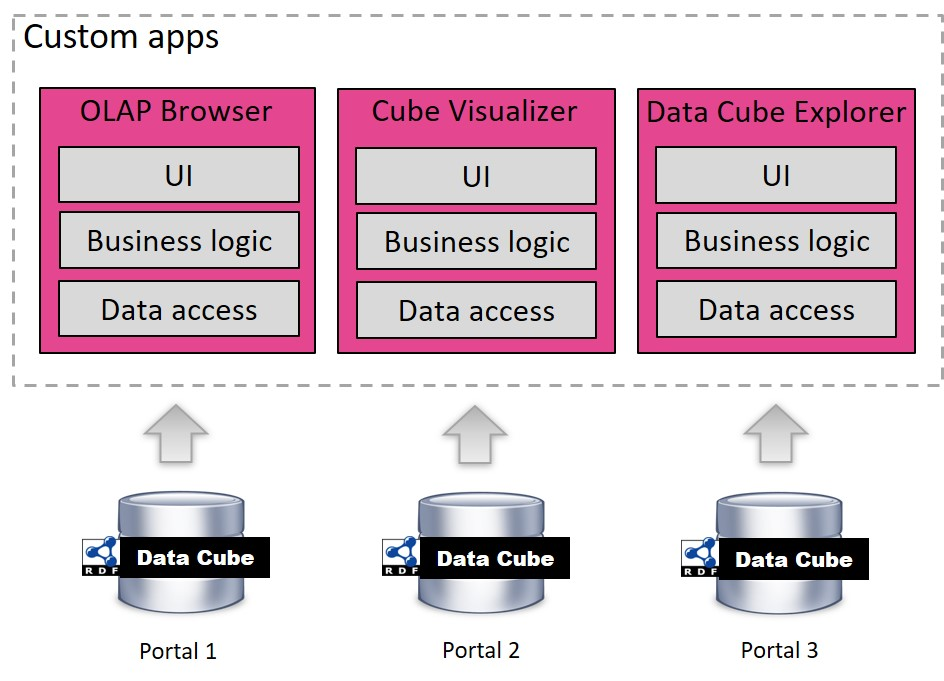
\includegraphics[width=110mm]{images/overview1.jpg}
  \end{center}
\caption{AS-IS overview}
\label{fig:overview1}
\end{figure}


\begin{figure}[h!]
  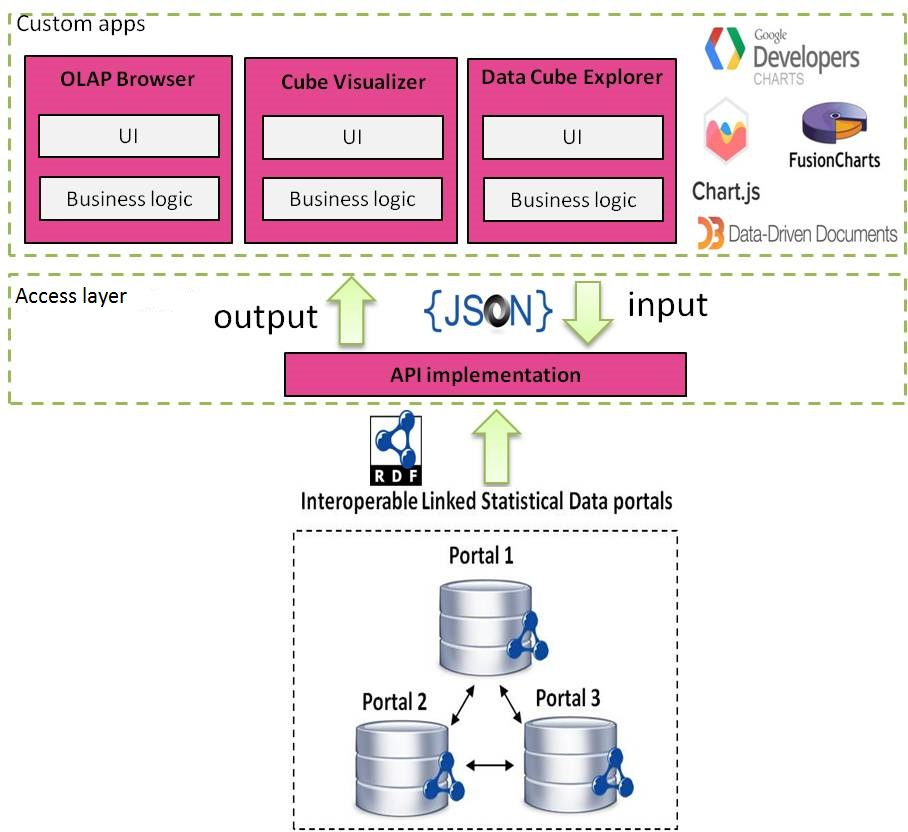
\includegraphics[width=110mm]{images/overview.jpg}
\caption{Solution overview}
\label{fig:overview}
\end{figure}





\section{Requirements and design criteria}\label{sec:reqs}

This section presents the functional and non-functional requirements and design criteria related to the Linked Open Statistical Data API.
A summary of the requirements is presented at table \ref{tbl:req}.

\begin{table}
\caption{Summary of API requirements}
\begin{tabular}{p{2cm}p{4cm}p{5.9cm}}
\hline\noalign{\smallskip}
\textbf{Type} & \textbf{Name} & \textbf{Description}\\
\noalign{\smallskip}
\hline
\noalign{\smallskip}
\multirow{3}{*}{functional} & Search data cubes & Search for data cubes at linked statistical data portals based on specified criteria\\\noalign{\smallskip}
 & Explore data cube structure & Having a cube at hand, get information about its structure (e.g. dimensions, measures, attributes)\\\noalign{\smallskip}
 & Slicing and filtering & Get a sub-set (slice) of cube observations based on user-defined criteria\\\noalign{\smallskip}\hline
\multirow{4}{*}{non-functional} & Easy of use & Provide a style of interaction that is familiar to web developers\\\noalign{\smallskip}
 & Uniform data access & Hide any discrepancies of published data cubes\\\noalign{\smallskip}
 & High performance & Provide responses fast even for demanding requests\\\noalign{\smallskip}
 & Extensibility & Enable the addition of new or the modification of existing functionality\\\noalign{\smallskip}
\hline
\end{tabular}
\label{tbl:req}
\end{table}

\subsection{Search data cubes}\label{sec:search}

The linked data web currently contains many published data cubes and their number still increases. Thus, applications need to search for cubes based on some criteria. For example, get cubes that measure unemployment, or get cubes for Greece. The search can be even more complex e.g. get cubes about unemployment in Greece after 2010. To fully exploit the cube searching functionality, the API ideally should search over the linked data web and not be limited to a single RDF store.

The search functionality can also be extended to support not only user specific criteria (as the previous examples), but also support the ``automatic" search of compatible cubes that could be processed together. For example, having a cube at hand search for other cubes that are compatible for combined statistical analysis, for visualisation of for browsing. The cube compatibility criteria is still an open issue and is out of the scope of this paper. 

\subsection{Explore data cube structure}

Once a cube has been identified (e.g. through the search functionality) the processing application (e.g. cube browser) needs to initialize the user interface or the analysis with information related to the cube structure. For example, populate drop-down menus with the cube dimensions and measures. The QB vocabulary clearly identifies the main elements of the structure that should be accessed through the API:
\begin{itemize}
\item Dataset meta-data. They include information like the label, description, issue date, publisher and license.
\item Dimensions. They include all the dimension properties of the cube (e.g. reference area, reference period).
\item Measures. They include all the measure properties of the cube (e.g. unemployment, poverty)
\item Attributes. They include all the attribute properties of the cube (e.g. unit of measure)
\item Dimension values. They include all the values of a dimension (e.g. male, female) that appear at the cube. 
\item Dimension levels. In the case of hierarchical data, dimension values are organized to hierarchical levels (e.g. region, district).
\item Attribute values. They include all the values of an attribute (e.g. euro, dollar) that appear at the cube. 
\end{itemize} 

Regarding the last three elements, the QB vocabulary does not offer a way to retrieve the values / levels directly from the structure. Thus the API should iterate over the cube observations, which is a time consuming task.

\subsection{Slicing and filtering}\label{sec:slice}

There are already methods available for downloading entire data cubes but people often want just small parts.  Whole cubes are often too big to be well-suited to interactive applications, and if the data updates frequently,  then it's important for people to be able to retrieve up-to-date extracts of the data, rather than keeping their own copies of full datasets up to date. The API should allow applications to take exactly the data they want by defining constrains (i.e. filters) to the dimension values. The API should support many filtering options including:
\begin{itemize}
\item Single values e.g. refPeriod=2010.
\item Multiple values e.g. refPeriod=[2010, 2011, 2012]
\item Ranges e.g refPeriod=[2010 ... 2015]
\item Greater/smaller than e.g. refPeriod$>$2010
\item Hierarchical data filtering e.g. refArea=``all council areas in Scotland"
\end{itemize}

In many cases, applications do not need all the requested data at once, because they process them at bunches. For example, a cube browser shows a part of the data allowing the user to navigate to the previous/next page of data. Thus, the API should support paging and ordering of the results. The ordering of the results can be in ascending or descending order based on one or more dimensions. However, in some cases lexicographical ordering is not appropriate (e.g. for the days of the week), thus other types of ordering should be applied.

\subsection{Easy of use}

Linked data offer many benefits to web developers, including the easy integration on the web. However, linked data technologies (i.e. RDF, SPARQL) are unfamiliar to many developers, thus creating many obstacles at their adoption. The purposes of the API is to exploit the advantages of linked data through a style of interaction that is familiar to web developers, thus helping them create data visualisations and applications.

The easy of use of an API is related both to the input of the API (API calls) and the out put. Regarding the input of the API there are mainly two design options: i) use a separate parameter for each required input and ii) model all the required input as a JSON object. The first option is post popular at existing APIs, while the second is more flexible and expressive. For example, it enables the expression of relations other than equality e.g. greater than (see Table \ref{tbl:apiinput}).

\begin{table}
\caption{Input of API: separate parameters vs JSON object}
\begin{tabular}{ll}
\hline\noalign{\smallskip}
\textbf{Separate parameters} & \textbf{Input as JSON}\\
\noalign{\smallskip}
\hline
\noalign{\smallskip}
\begin{minipage}[t]{2.2in}
 \begin{verbatim} 
GET /slice?dataset=home-care&
            gender=male         
\end{verbatim}
\end{minipage}
&
 \begin{minipage}[t]{2.3in}
\begin{verbatim} 
{"dataset": "home-care",
 "filter": {
   "gender": "male"
}}
\end{verbatim}
\end{minipage}\\\noalign{\smallskip}
\begin{minipage}[t]{2.2in}
 \begin{verbatim} 
Cannot be expressed                    
\end{verbatim}
\end{minipage}
&
\begin{minipage}[t]{2.3in}
\begin{verbatim} 
{"dataset": "home-care",
 "filter": {
   "gender": "male"
   "age": { "greater-than": 50}
}}
\end{verbatim}
\end{minipage}\\\noalign{\smallskip}
\hline
\end{tabular}
\label{tbl:apiinput}
\end{table}


Regarding the output of the API, JSON is a popular, easy to use format. Usually, applications and visualizations do not require an n-array/ tabular response (e.g. JSON-stat); an array of observations is sufficient and more straightforward. In case that a tabular response is required, then it can easily be constructed from the observations. An example of a JSON code that could represents an array of observations is presented below.

\begin{verbatim} 
{ "observations": [ 
    {"gender"       : "male", 
     "age"          : "55-65", 
     "refPeriod"    : "2016",
     "refArea"      : "Scotland",
     "unemployment" : "4.3",
     "unit"         : "percent"}, 
    {"gender"       : "female", 
     "age"          : "55-65", 
     "refPeriod"    : "2016",
     "refArea"      : "Scotland",
     "unemployment" : "4.7",
     "unit"         : "percent"},
     ...
]}
\end{verbatim}

Finally, JSON-LD representation can be used both at the input and output of the API format in order to represent linked data.

\subsection{Uniform data access}

Currently many linked data cubes have been published through official data portals, however a lot of them adopt different publishing practices. As a result, only case specific applications can be created that assume data published in a specific way. The API should work on top of any of these data, offering uniform access to the data and hide any discrepancies. Obviously, this will require different API implementations to comply with the different publishing practices. However, using the API as the main way to deliver data, will reduce the need for data publishers to maintain public SPARQL endpoints.

Ideally, the standardization of the API specification will also lead to the formulation of an application profile for the QB vocabulary. The profile will include best practices that can be used by data publishers to provide data in a compatible way, facilitating in this way the development of generic linked data cube applications.

\subsection{High performance}

The volume of data published as linked data cubes is big, reaching the magnitude of million triples per cube. Thus, SPARQL queries that iterate over all the observations tend to be slow. For example, a query to get all the dimension values that appear at a cube needs to iterate over all the observations. As a result, applications that use such queries seem to be non-responsive. 

The API can improve performance of demanding SPARQL queries through efficient caching of the responses. The caching policy (e.g. Least Recently Used, Least Frequently Used) plays an important role at the performance improvement. Note that caching of API responses is much easier that caching of arbitrary SPARQL queries. 

Another task that can improve the performance of the API is the pre-computation of aggregations: i) across a dimension of the cube e.g. compute the SUM of the sales over time and thus ignore the time dimension of the cube and ii) across a hierarchy e.g. if a cube contains the election results at municipality level, then aggregations can be computed at region and at country level. The pre-computation of the aggregations facilitates the execution of queries, because there in not need to compute the aggregations on-the-fly when requested. 


\subsection{Extensibility}

Finally, a requirement of the API is to be extensible, thus take future growth into consideration minimizing the effort required for the extension. Extensions can be implemented through the :
\begin{itemize}
\item addition of new functionality e.g. while the initial aim is to build an API on top of RDF databases, other kinds of database could be used, enabling flexibility and innovation
\item modification of existing functionality e.g. support modified search (see section \ref{sec:search}) of filtering options (see section \ref{sec:slice}).
\end{itemize} 


\section{Implementation}\label{sec:impl}


The API implementation\footnote{https://github.com/OpenGovIntelligence/json-qb-api-implementation} aims to provide an easy to use API for web developers that use statistical data stored in the form of RDF Data cubes. It  can be installed on top of any RDF repository and offer basic and advanced operations on RDF Data cubes assuming that: i) they are stored using the RDF Data Cube Vocabulary, ii) they follow a specific application profile (common practices) and iii) are accessible through a SPARQL endpoint.  All the functionality is offered through simple REST calls. The API translates each call to a SPARQL query that is executed at the linked data cubes. The returned results are always transformed  in JSON format 

The implementation of the API uses the following technologies:
\begin{itemize}
\item Jersey  framework for the implementation of the RESTful services. Jersey is an implementation of the JAX-RS  Reference Implementation. 
\item SPARQL  for querying the RDF repositories. 
\item Rdf4j  Java framework for processing RDF data 
\item Gson  Java library to serialize Java Objects into their JSON representation  
\end{itemize}



\begin{table}
\caption{Example API calls}
\begin{tabular}{|l|l|}
\hline
\multicolumn{2}{|c|}{\textbf{Dimensions}}\\

\hline
API call &
\begin{minipage}[t]{4.5in}
 \begin{verbatim} 
GET /dimensions?dataset=http://example.com/cube/unemployment         
\end{verbatim}
\end{minipage}\\\hline

SPARQL query  &
\begin{minipage}[t]{4.5in}
 \begin{verbatim} 
PREFIX qb: http://purl.org/linked-data/cube#
PREFIX rdfs: http://www.w3.org/2000/01/rdf-schema#
PREFIX ex: http://example.com/cube/
select distinct ?dim ?label where {
    ex:unemployment qb:structure ?dsd.
    ?dsd qb:component  ?cs.
    ?cs qb:dimension ?dim.
    ?dim rdfs:label ?label.} 
\end{verbatim}
\end{minipage}\\ \hline

JSON result &
\begin{minipage}[t]{4.5in}
 \begin{verbatim} 
{"dimensions":[
  {"@id":  "http://example.com/dimension/refArea",
   "label":"Reference area"},
  {"@id":  "http://example.com/dimension/refPeriod",
   "label":"Reference period"},
   ....
 ]
}  
\end{verbatim}
\end{minipage}\\\hline



\multicolumn{2}{|c|}{\textbf{Slice}}\\

\hline
API call &
\begin{minipage}[t]{4.5in}
 \begin{verbatim} 
GET /slice
\end{verbatim}
\end{minipage}\\\hline

SPARQL query  &
\begin{minipage}[t]{4.5in}
 \begin{verbatim} 
XXX
\end{verbatim}
\end{minipage}\\ \hline

JSON result &
\begin{minipage}[t]{4.5in}
 \begin{verbatim} 
YYY 
\end{verbatim}
\end{minipage}\\\hline


\end{tabular}
\label{tbl:apiexamplecall}
\end{table}




++ easy app creation++ image cube visualiser!


\section{Conclusion}\label{sec:conclusion}



\bibliographystyle{splncs03}


\bibliography{qbbibfile}   % name your BibTeX data base


\end{document}


